
\begin{figure}[h]
\centering
\tikzset{every picture/.style={line width=0.75pt}} %set default line width to 0.75pt        

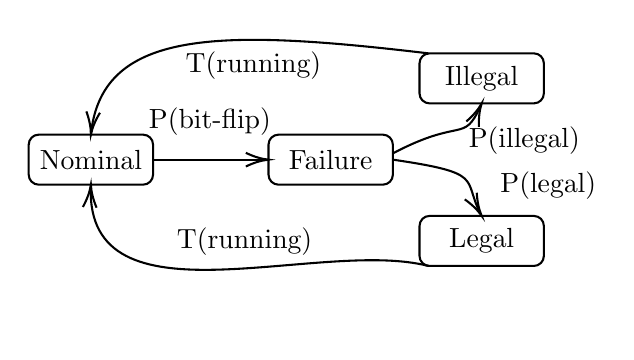
\begin{tikzpicture}[x=0.75pt,y=0.75pt,yscale=-1,xscale=1]
%uncomment if require: \path (0,235); %set diagram left start at 0, and has height of 235

%Rounded Rect [id:dp4097096976762369] 
\draw   (10,64.69) .. controls (10,62.02) and (12.16,59.87) .. (14.82,59.87) -- (65.09,59.87) .. controls (67.75,59.87) and (69.91,62.02) .. (69.91,64.69) -- (69.91,79.15) .. controls (69.91,81.81) and (67.75,83.97) .. (65.09,83.97) -- (14.82,83.97) .. controls (12.16,83.97) and (10,81.81) .. (10,79.15) -- cycle ;
%Rounded Rect [id:dp2835435765541303] 
\draw   (125.54,64.69) .. controls (125.54,62.02) and (127.7,59.87) .. (130.36,59.87) -- (180.63,59.87) .. controls (183.29,59.87) and (185.45,62.02) .. (185.45,64.69) -- (185.45,79.15) .. controls (185.45,81.81) and (183.29,83.97) .. (180.63,83.97) -- (130.36,83.97) .. controls (127.7,83.97) and (125.54,81.81) .. (125.54,79.15) -- cycle ;
%Rounded Rect [id:dp5805736774223651] 
\draw   (198.29,25.52) .. controls (198.29,22.86) and (200.45,20.7) .. (203.11,20.7) -- (253.38,20.7) .. controls (256.04,20.7) and (258.2,22.86) .. (258.2,25.52) -- (258.2,39.98) .. controls (258.2,42.64) and (256.04,44.8) .. (253.38,44.8) -- (203.11,44.8) .. controls (200.45,44.8) and (198.29,42.64) .. (198.29,39.98) -- cycle ;
%Rounded Rect [id:dp8614575685420135] 
\draw   (198.29,103.85) .. controls (198.29,101.19) and (200.45,99.03) .. (203.11,99.03) -- (253.38,99.03) .. controls (256.04,99.03) and (258.2,101.19) .. (258.2,103.85) -- (258.2,118.31) .. controls (258.2,120.97) and (256.04,123.13) .. (253.38,123.13) -- (203.11,123.13) .. controls (200.45,123.13) and (198.29,120.97) .. (198.29,118.31) -- cycle ;
%Curve Lines [id:da16079762072366677] 
\draw    (185.45,68.9) .. controls (218.66,51.37) and (219.45,64.08) .. (227.48,46.52) ;
\draw [shift={(228.25,44.8)}, rotate = 113.59] [color={rgb, 255:red, 0; green, 0; blue, 0 }  ][line width=0.75]    (10.93,-3.29) .. controls (6.95,-1.4) and (3.31,-0.3) .. (0,0) .. controls (3.31,0.3) and (6.95,1.4) .. (10.93,3.29)   ;
%Curve Lines [id:da04663923009445026] 
\draw    (185.45,71.92) .. controls (229.87,78.4) and (219.12,81.01) .. (227.42,97.46) ;
\draw [shift={(228.25,99.03)}, rotate = 241.15] [color={rgb, 255:red, 0; green, 0; blue, 0 }  ][line width=0.75]    (10.93,-3.29) .. controls (6.95,-1.4) and (3.31,-0.3) .. (0,0) .. controls (3.31,0.3) and (6.95,1.4) .. (10.93,3.29)   ;
%Straight Lines [id:da44802200900780054] 
\draw    (69.91,71.92) -- (123.54,71.92) ;
\draw [shift={(125.54,71.92)}, rotate = 180] [color={rgb, 255:red, 0; green, 0; blue, 0 }  ][line width=0.75]    (10.93,-3.29) .. controls (6.95,-1.4) and (3.31,-0.3) .. (0,0) .. controls (3.31,0.3) and (6.95,1.4) .. (10.93,3.29)   ;
%Curve Lines [id:da03387373961296125] 
\draw    (202.57,20.7) .. controls (102.59,8.83) and (46.22,8.86) .. (40.12,58.35) ;
\draw [shift={(39.96,59.87)}, rotate = 275.75] [color={rgb, 255:red, 0; green, 0; blue, 0 }  ][line width=0.75]    (10.93,-3.29) .. controls (6.95,-1.4) and (3.31,-0.3) .. (0,0) .. controls (3.31,0.3) and (6.95,1.4) .. (10.93,3.29)   ;
%Curve Lines [id:da005071296130858216] 
\draw    (202.57,123.13) .. controls (149.77,109.55) and (37.45,154.22) .. (39.91,85.02) ;
\draw [shift={(39.96,83.97)}, rotate = 92.95] [color={rgb, 255:red, 0; green, 0; blue, 0 }  ][line width=0.75]    (10.93,-3.29) .. controls (6.95,-1.4) and (3.31,-0.3) .. (0,0) .. controls (3.31,0.3) and (6.95,1.4) .. (10.93,3.29)   ;

% Text Node
\draw (39.96,71.92) node   [align=left] {Nominal};
% Text Node
\draw (155.5,71.92) node   [align=left] {Failure};
% Text Node
\draw (228.25,32.75) node   [align=left] {Illegal};
% Text Node
\draw (228.25,111.08) node   [align=left] {Legal};
% Text Node
\draw (248.79,62.58) node   [align=left] {P(illegal)};
% Text Node
\draw (260.34,84.27) node   [align=left] {P(legal)};
% Text Node
\draw (118.27,26.43) node   [align=left] {T(running)};
% Text Node
\draw (113.99,111.38) node   [align=left] {T(running)};
% Text Node
\draw (97.3,53.54) node   [align=left] {P(bit-flip)};

\end{tikzpicture}
\caption{Altarica Dysfunctional Model}
\label{altarica-model}
\end{figure}
